% !TeX spellcheck = IT

% Chapter heading images should have a 2:1 width:height ratio,

%----------------------------------------------------------------------------------------
%	PACKAGES AND OTHER DOCUMENT CONFIGURATIONS
%----------------------------------------------------------------------------------------

\documentclass[11pt,fleqn]{book} % Default font size and left-justified equations

\usepackage[top=3cm,bottom=3cm,left=3cm,right=3cm,headsep=10pt,a4paper]{geometry} % Page margins

\usepackage{xcolor} % Required for specifying colors by name
\definecolor{ocre}{RGB}{52,177,201} % Define the orange color used for highlighting throughout the book

% Font Settings
\usepackage{avant} % Use the Avantgarde font for headings
%\usepackage{times} % Use the Times font for headings
\usepackage{mathptmx} % Use the Adobe Times Roman as the default text font together with math symbols from the Sym­bol, Chancery and Com­puter Modern fonts

\usepackage{microtype} % Slightly tweak font spacing for aesthetics
\usepackage[utf8]{inputenc} % Required for including letters with accents
\usepackage[T1]{fontenc} % Use 8-bit encoding that has 256 glyphs

% Bibliography
%\usepackage[style=alphabetic,sorting=nyt,sortcites=true,autopunct=true,babel=hyphen,hyperref=true,abbreviate=false,backref=true,backend=biber]{autolang}
%\addbibresource{bibliography.bib} % BibTeX bibliography file
%\defbibheading{bibempty}{}

%%%%%%%%%%%%%%%%%%%%%%%%%%%%%%%%%%%%%%%%%
% The Legrand Orange Book
% Structural Definitions File
% Version 2.0 (9/2/15)
%
% Original author:
% Mathias Legrand (legrand.mathias@gmail.com) with modifications by:
% Vel (vel@latextemplates.com)
% 
% This file has been downloaded from:
% http://www.LaTeXTemplates.com
%
% License:
% CC BY-NC-SA 3.0 (http://creativecommons.org/licenses/by-nc-sa/3.0/)
%
%%%%%%%%%%%%%%%%%%%%%%%%%%%%%%%%%%%%%%%%%

%----------------------------------------------------------------------------------------
%	VARIOUS REQUIRED PACKAGES AND CONFIGURATIONS
%----------------------------------------------------------------------------------------

\usepackage[top=3cm,bottom=3cm,left=3cm,right=3cm,headsep=10pt,a4paper]{geometry} % Page margins

\usepackage{graphicx} % Required for including pictures
\graphicspath{{Pictures/}} % Specifies the directory where pictures are stored

\usepackage{lipsum} % Inserts dummy text

\usepackage{tikz} % Required for drawing custom shapes

\usepackage[italian]{babel} % English language/hyphenation

\usepackage{enumitem} % Customize lists
\setlist{nolistsep} % Reduce spacing between bullet points and numbered lists

\usepackage{booktabs} % Required for nicer horizontal rules in tables

\usepackage{xcolor} % Required for specifying colors by name
\definecolor{ocre}{RGB}{243,102,25} % Define the orange color used for highlighting throughout the book
\definecolor{blue}{RGB}{50,153,255}
%----------------------------------------------------------------------------------------
%	FONTS
%----------------------------------------------------------------------------------------

\usepackage{avant} % Use the Avantgarde font for headings
%\usepackage{times} % Use the Times font for headings
\usepackage{mathptmx} % Use the Adobe Times Roman as the default text font together with math symbols from the Sym­bol, Chancery and Com­puter Modern fonts

\usepackage{microtype} % Slightly tweak font spacing for aesthetics
\usepackage[utf8]{inputenc} % Required for including letters with accents
\usepackage[T1]{fontenc} % Use 8-bit encoding that has 256 glyphs

%----------------------------------------------------------------------------------------
%	BIBLIOGRAPHY AND INDEX
%----------------------------------------------------------------------------------------

\usepackage[style=numeric,citestyle=numeric,sorting=nyt,sortcites=true,autopunct=true,babel=hyphen,hyperref=true,abbreviate=false,backref=true,backend=biber]{biblatex}
\addbibresource{bibliography.bib} % BibTeX bibliography file
\defbibheading{bibempty}{}

\usepackage{calc} % For simpler calculation - used for spacing the index letter headings correctly
\usepackage{makeidx} % Required to make an index
\makeindex % Tells LaTeX to create the files required for indexing

%----------------------------------------------------------------------------------------
%	MAIN TABLE OF CONTENTS
%----------------------------------------------------------------------------------------

\usepackage{titletoc} % Required for manipulating the table of contents

\contentsmargin{0cm} % Removes the default margin

% Part text styling
\titlecontents{part}[0cm]
{\addvspace{20pt}\centering\large\bfseries}
{}
{}
{}

% Chapter text styling
\titlecontents{chapter}[1.30cm] % Indentation
{\addvspace{12pt}\large\sffamily\bfseries} % Spacing and font options for chapters
{\color{blue}\contentslabel[\Large\thecontentslabel]{1.30cm}\color{blue}} % Chapter number
{\color{blue}}  
{\color{blue!70}\normalsize\;\titlerule*[.5pc]{.}\;\thecontentspage} % Page number

% Section text styling
\titlecontents{section}[1.20cm] % Indentation
{\addvspace{3pt}\sffamily\bfseries} % Spacing and font options for sections
{\color{ocre}\contentslabel[\thecontentslabel]{1.20cm}\color{black}} % Chapter number
{\color{ocre}}  
{\color{ocre!70}\normalsize\;\titlerule*[.5pc]{.}\;\thecontentspage}

% Subsection text styling
\titlecontents{subsection}[1.20cm] % Indentation
{\addvspace{1pt}\sffamily\small} % Spacing and font options for subsections
{\contentslabel[\thecontentslabel]{1.20cm}} % Subsection number
{}
{\ \titlerule*[.5pc]{.}\;\thecontentspage} % Page number
[]

% List of figures
\titlecontents{figure}[0em]
{\addvspace{-5pt}\sffamily}
{\thecontentslabel\hspace*{1em}}
{}
{\ \titlerule*[.5pc]{.}\;\thecontentspage}
[]

% List of tables
\titlecontents{table}[0em]
{\addvspace{-5pt}\sffamily}
{\thecontentslabel\hspace*{1em}}
{}
{\ \titlerule*[.5pc]{.}\;\thecontentspage}
[]

%----------------------------------------------------------------------------------------
%	MINI TABLE OF CONTENTS IN PART HEADS
%----------------------------------------------------------------------------------------

% Chapter text styling
\titlecontents{lchapter}[0em] % Indenting
{\addvspace{15pt}\large\sffamily\bfseries} % Spacing and font options for chapters
{\color{ocre}\contentslabel[\Large\thecontentslabel]{1.25cm}\color{ocre}} % Chapter number
{}  
{\color{ocre}\normalsize\sffamily\bfseries\;\titlerule*[.5pc]{.}\;\thecontentspage} % Page number

% Section text styling
\titlecontents{lsection}[0em] % Indenting
{\sffamily\small} % Spacing and font options for sections
{\contentslabel[\thecontentslabel]{1.25cm}} % Section number
{}
{}

% Subsection text styling
\titlecontents{lsubsection}[.5em] % Indentation
{\normalfont\footnotesize\sffamily} % Font settings
{}
{}
{}

%----------------------------------------------------------------------------------------
%	PAGE HEADERS
%----------------------------------------------------------------------------------------

\usepackage{fancyhdr} % Required for header and footer configuration

\pagestyle{fancy}
\renewcommand{\chaptermark}[1]{\markboth{\sffamily\normalsize\bfseries\chaptername\ \thechapter.\ #1}{}} % Chapter text font settings
\renewcommand{\sectionmark}[1]{\markright{\sffamily\normalsize\thesection\hspace{5pt}#1}{}} % Section text font settings
\fancyhf{} \fancyhead[LE,RO]{\sffamily\normalsize\thepage} % Font setting for the page number in the header
\fancyhead[LO]{\rightmark} % Print the nearest section name on the left side of odd pages
\fancyhead[RE]{\leftmark} % Print the current chapter name on the right side of even pages
\renewcommand{\headrulewidth}{0.5pt} % Width of the rule under the header
\addtolength{\headheight}{2.5pt} % Increase the spacing around the header slightly
\renewcommand{\footrulewidth}{0pt} % Removes the rule in the footer
\fancypagestyle{plain}{\fancyhead{}\renewcommand{\headrulewidth}{0pt}} % Style for when a plain pagestyle is specified

% Removes the header from odd empty pages at the end of chapters
\makeatletter
\renewcommand{\cleardoublepage}{
\clearpage\ifodd\c@page\else
\hbox{}
\vspace*{\fill}
\thispagestyle{empty}
%\newpage
\fi}

%----------------------------------------------------------------------------------------
%	THEOREM STYLES
%----------------------------------------------------------------------------------------

\usepackage{amsmath,amsfonts,amssymb,amsthm} % For math equations, theorems, symbols, etc

\newcommand{\intoo}[2]{\mathopen{]}#1\,;#2\mathclose{[}}
\newcommand{\ud}{\mathop{\mathrm{{}d}}\mathopen{}}
\newcommand{\intff}[2]{\mathopen{[}#1\,;#2\mathclose{]}}
\newtheorem{notation}{Notation}[chapter]

% Boxed/framed environments
\newtheoremstyle{ocrenumbox}% % Theorem style name
{0pt}% Space above
{0pt}% Space below
{\normalfont}% % Body font
{}% Indent amount
{\small\bf\sffamily\color{ocre}}% % Theorem head font
{\;}% Punctuation after theorem head
{0.25em}% Space after theorem head
{\small\sffamily\color{ocre}\thmname{#1}\nobreakspace\thmnumber{\@ifnotempty{#1}{}\@upn{#2}}% Theorem text (e.g. Theorem 2.1)
\thmnote{\nobreakspace\the\thm@notefont\sffamily\bfseries\color{black}---\nobreakspace#3.}} % Optional theorem note
\renewcommand{\qedsymbol}{$\blacksquare$}% Optional qed square

\newtheoremstyle{blacknumex}% Theorem style name
{5pt}% Space above
{5pt}% Space below
{\normalfont}% Body font
{} % Indent amount
{\small\bf\sffamily}% Theorem head font
{\;}% Punctuation after theorem head
{0.25em}% Space after theorem head
{\small\sffamily{\tiny\ensuremath{\blacksquare}}\nobreakspace\thmname{#1}\nobreakspace\thmnumber{\@ifnotempty{#1}{}\@upn{#2}}% Theorem text (e.g. Theorem 2.1)
\thmnote{\nobreakspace\the\thm@notefont\sffamily\bfseries---\nobreakspace#3.}}% Optional theorem note

\newtheoremstyle{blacknumbox} % Theorem style name
{0pt}% Space above
{0pt}% Space below
{\normalfont}% Body font
{}% Indent amount
{\small\bf\sffamily}% Theorem head font
{\;}% Punctuation after theorem head
{0.25em}% Space after theorem head
{\small\sffamily\thmname{#1}\nobreakspace\thmnumber{\@ifnotempty{#1}{}\@upn{#2}}% Theorem text (e.g. Theorem 2.1)
\thmnote{\nobreakspace\the\thm@notefont\sffamily\bfseries---\nobreakspace#3.}}% Optional theorem note

% Non-boxed/non-framed environments
\newtheoremstyle{ocrenum}% % Theorem style name
{5pt}% Space above
{5pt}% Space below
{\normalfont}% % Body font
{}% Indent amount
{\small\bf\sffamily\color{ocre}}% % Theorem head font
{\;}% Punctuation after theorem head
{0.25em}% Space after theorem head
{\small\sffamily\color{ocre}\thmname{#1}\nobreakspace\thmnumber{\@ifnotempty{#1}{}\@upn{#2}}% Theorem text (e.g. Theorem 2.1)
\thmnote{\nobreakspace\the\thm@notefont\sffamily\bfseries\color{black}---\nobreakspace#3.}} % Optional theorem note
\renewcommand{\qedsymbol}{$\blacksquare$}% Optional qed square
\makeatother

% Defines the theorem text style for each type of theorem to one of the three styles above
\newcounter{dummy} 
\numberwithin{dummy}{section}
\theoremstyle{ocrenumbox}
\newtheorem{theoremeT}[dummy]{Theorem}
\newtheorem{problem}{Problem}[chapter]
\newtheorem{exerciseT}{Exercise}[chapter]
\theoremstyle{blacknumex}
\newtheorem{exampleT}{Example}[chapter]
\theoremstyle{blacknumbox}
\newtheorem{vocabulary}{Vocabulary}[chapter]
\newtheorem{definitionT}{Definition}[section]
\newtheorem{corollaryT}[dummy]{Corollary}
\theoremstyle{ocrenum}
\newtheorem{proposition}[dummy]{Proposition}

%----------------------------------------------------------------------------------------
%	DEFINITION OF COLORED BOXES
%----------------------------------------------------------------------------------------

\RequirePackage[framemethod=default]{mdframed} % Required for creating the theorem, definition, exercise and corollary boxes

% Theorem box
\newmdenv[skipabove=7pt,
skipbelow=7pt,
backgroundcolor=black!5,
linecolor=ocre,
innerleftmargin=5pt,
innerrightmargin=5pt,
innertopmargin=5pt,
leftmargin=0cm,
rightmargin=0cm,
innerbottommargin=5pt]{tBox}

% Exercise box	  
\newmdenv[skipabove=7pt,
skipbelow=7pt,
rightline=false,
leftline=true,
topline=false,
bottomline=false,
backgroundcolor=ocre!10,
linecolor=ocre,
innerleftmargin=5pt,
innerrightmargin=5pt,
innertopmargin=5pt,
innerbottommargin=5pt,
leftmargin=0cm,
rightmargin=0cm,
linewidth=4pt]{eBox}	

% Definition box
\newmdenv[skipabove=7pt,
skipbelow=7pt,
rightline=false,
leftline=true,
topline=false,
bottomline=false,
linecolor=ocre,
innerleftmargin=5pt,
innerrightmargin=5pt,
innertopmargin=0pt,
leftmargin=0cm,
rightmargin=0cm,
linewidth=4pt,
innerbottommargin=0pt]{dBox}	

% Corollary box
\newmdenv[skipabove=7pt,
skipbelow=7pt,
rightline=false,
leftline=true,
topline=false,
bottomline=false,
linecolor=gray,
backgroundcolor=black!5,
innerleftmargin=5pt,
innerrightmargin=5pt,
innertopmargin=5pt,
leftmargin=0cm,
rightmargin=0cm,
linewidth=4pt,
innerbottommargin=5pt]{cBox}

% Creates an environment for each type of theorem and assigns it a theorem text style from the "Theorem Styles" section above and a colored box from above
\newenvironment{theorem}{\begin{tBox}\begin{theoremeT}}{\end{theoremeT}\end{tBox}}
\newenvironment{exercise}{\begin{eBox}\begin{exerciseT}}{\hfill{\color{ocre}\tiny\ensuremath{\blacksquare}}\end{exerciseT}\end{eBox}}				  
\newenvironment{definition}{\begin{dBox}\begin{definitionT}}{\end{definitionT}\end{dBox}}	
\newenvironment{example}{\begin{exampleT}}{\hfill{\tiny\ensuremath{\blacksquare}}\end{exampleT}}		
\newenvironment{corollary}{\begin{cBox}\begin{corollaryT}}{\end{corollaryT}\end{cBox}}	

%----------------------------------------------------------------------------------------
%	REMARK ENVIRONMENT
%----------------------------------------------------------------------------------------

\newenvironment{remark}{\par\vspace{10pt}\small % Vertical white space above the remark and smaller font size
\begin{list}{}{
\leftmargin=35pt % Indentation on the left
\rightmargin=25pt}\item\ignorespaces % Indentation on the right
\makebox[-2.5pt]{\begin{tikzpicture}[overlay]
\node[draw=blue!60,line width=1pt,circle,fill=ocre!25,font=\sffamily\bfseries,inner sep=2pt,outer sep=0pt] at (-15pt,0pt){\textcolor{blue}{R}};\end{tikzpicture}} % Orange R in a circle
\advance\baselineskip -1pt}{\end{list}\vskip5pt} % Tighter line spacing and white space after remark

%----------------------------------------------------------------------------------------
%	SECTION NUMBERING IN THE MARGIN
%----------------------------------------------------------------------------------------

\makeatletter
\renewcommand{\@seccntformat}[1]{\llap{\textcolor{ocre}{\csname the#1\endcsname}\hspace{1em}}}                    
\renewcommand{\section}{\@startsection{section}{1}{\z@}
{-4ex \@plus -1ex \@minus -.4ex}
{1ex \@plus.2ex }
{\normalfont\large\sffamily\bfseries}}
\renewcommand{\subsection}{\@startsection {subsection}{2}{\z@}
{-3ex \@plus -0.1ex \@minus -.4ex}
{0.5ex \@plus.2ex }
{\normalfont\sffamily\bfseries}}
\renewcommand{\subsubsection}{\@startsection {subsubsection}{3}{\z@}
{-2ex \@plus -0.1ex \@minus -.2ex}
{.2ex \@plus.2ex }
{\normalfont\small\sffamily\bfseries}}                        
\renewcommand\paragraph{\@startsection{paragraph}{4}{\z@}
{-2ex \@plus-.2ex \@minus .2ex}
{.1ex}
{\normalfont\small\sffamily\bfseries}}

%----------------------------------------------------------------------------------------
%	PART HEADINGS
%----------------------------------------------------------------------------------------

% numbered part in the table of contents
\newcommand{\@mypartnumtocformat}[2]{%
\setlength\fboxsep{0pt}%
\noindent\colorbox{ocre!20}{\strut\parbox[c][.7cm]{\ecart}{\color{ocre!70}\Large\sffamily\bfseries\centering#1}}\hskip\esp\colorbox{ocre!40}{\strut\parbox[c][.7cm]{\linewidth-\ecart-\esp}{\Large\sffamily\centering#2}}}%
%%%%%%%%%%%%%%%%%%%%%%%%%%%%%%%%%%
% unnumbered part in the table of contents
\newcommand{\@myparttocformat}[1]{%
\setlength\fboxsep{0pt}%
\noindent\colorbox{ocre!40}{\strut\parbox[c][.7cm]{\linewidth}{\Large\sffamily\centering#1}}}%
%%%%%%%%%%%%%%%%%%%%%%%%%%%%%%%%%%
\newlength\esp
\setlength\esp{4pt}
\newlength\ecart
\setlength\ecart{1.2cm-\esp}
\newcommand{\thepartimage}{}%
\newcommand{\partimage}[1]{\renewcommand{\thepartimage}{#1}}%
\def\@part[#1]#2{%
\ifnum \c@secnumdepth >-2\relax%
\refstepcounter{part}%
\addcontentsline{toc}{part}{\texorpdfstring{\protect\@mypartnumtocformat{\thepart}{#1}}{\partname~\thepart\ ---\ #1}}
\else%
\addcontentsline{toc}{part}{\texorpdfstring{\protect\@myparttocformat{#1}}{#1}}%
\fi%
\startcontents%
\markboth{}{}%
{\thispagestyle{empty}%
\begin{tikzpicture}[remember picture,overlay]%
\node at (current page.north west){\begin{tikzpicture}[remember picture,overlay]%	
\fill[ocre!20](0cm,0cm) rectangle (\paperwidth,-\paperheight);
\node[anchor=north] at (4cm,-3.25cm){\color{ocre!40}\fontsize{220}{100}\sffamily\bfseries\thepart}; 
\node[anchor=south east] at (\paperwidth-1cm,-\paperheight+1cm){\parbox[t][][t]{8.5cm}{
\printcontents{l}{0}{\setcounter{tocdepth}{1}}%
}};
\node[anchor=north east] at (\paperwidth-1.5cm,-3.25cm){\parbox[t][][t]{15cm}{\strut\raggedleft\color{white}\fontsize{30}{30}\sffamily\bfseries#2}};
\end{tikzpicture}};
\end{tikzpicture}}%
\@endpart}
\def\@spart#1{%
\startcontents%
\phantomsection
{\thispagestyle{empty}%
\begin{tikzpicture}[remember picture,overlay]%
\node at (current page.north west){\begin{tikzpicture}[remember picture,overlay]%	
\fill[ocre!20](0cm,0cm) rectangle (\paperwidth,-\paperheight);
\node[anchor=north east] at (\paperwidth-1.5cm,-3.25cm){\parbox[t][][t]{15cm}{\strut\raggedleft\color{white}\fontsize{30}{30}\sffamily\bfseries#1}};
\end{tikzpicture}};
\end{tikzpicture}}
\addcontentsline{toc}{part}{\texorpdfstring{%
\setlength\fboxsep{0pt}%
\noindent\protect\colorbox{ocre!40}{\strut\protect\parbox[c][.7cm]{\linewidth}{\Large\sffamily\protect\centering #1\quad\mbox{}}}}{#1}}%
\@endpart}
\def\@endpart{\vfil\newpage
\if@twoside
\if@openright
\null
\thispagestyle{empty}%
\newpage
\fi
\fi
\if@tempswa
\twocolumn
\fi}

%----------------------------------------------------------------------------------------
%	CHAPTER HEADINGS
%----------------------------------------------------------------------------------------

% A switch to conditionally include a picture, implemented by  Christian Hupfer
\newif\ifusechapterimage
\usechapterimagetrue
\newcommand{\thechapterimage}{}%
\newcommand{\chapterimage}[1]{\ifusechapterimage\renewcommand{\thechapterimage}{#1}\fi}%
\newcommand{\autodot}{.}
\def\@makechapterhead#1{%
{\parindent \z@ \raggedright \normalfont
\ifnum \c@secnumdepth >\m@ne
\if@mainmatter
\begin{tikzpicture}[remember picture,overlay]
\node at (current page.north west)
{\begin{tikzpicture}[remember picture,overlay]
\node[anchor=north west,inner sep=0pt] at (0,0) {\ifusechapterimage\includegraphics[width=\paperwidth]{\thechapterimage}\fi};
\draw[anchor=west] (\Gm@lmargin,-9cm) node [line width=2pt,rounded corners=15pt,draw=blue,fill=white,fill opacity=0.7,inner sep=16pt]{\strut\makebox[22cm]{}};
\draw[anchor=west] (\Gm@lmargin+.3cm,-9cm) node {\huge\sffamily\bfseries\color{blue}\thechapter\autodot~#1\strut};
\end{tikzpicture}};
\end{tikzpicture}
\else
\begin{tikzpicture}[remember picture,overlay]
\node at (current page.north west)
{\begin{tikzpicture}[remember picture,overlay]
\node[anchor=north west,inner sep=0pt] at (0,0) {\ifusechapterimage\includegraphics[width=\paperwidth]{\thechapterimage}\fi};
\draw[anchor=west] (\Gm@lmargin,-9cm) node [line width=2pt,rounded corners=15pt,draw=blue,fill=white,fill opacity=0.7,inner sep=16pt]{\strut\makebox[22cm]{}};
\draw[anchor=west] (\Gm@lmargin+.3cm,-9cm) node {\huge\sffamily\bfseries\color{blue}#1\strut};
\end{tikzpicture}};
\end{tikzpicture}
\fi\fi\par\vspace*{270\p@}}}

%-------------------------------------------

\def\@makeschapterhead#1{%
\begin{tikzpicture}[remember picture,overlay]
\node at (current page.north west)
{\begin{tikzpicture}[remember picture,overlay]
\node[anchor=north west,inner sep=0pt] at (0,0) {\ifusechapterimage\includegraphics[width=\paperwidth]{\thechapterimage}\fi};
\draw[anchor=west] (\Gm@lmargin,-9cm) node [line width=2pt,rounded corners=15pt,draw=blue,fill=white,fill opacity=0.7,inner sep=16pt]{\strut\makebox[22cm]{}};
\draw[anchor=west] (\Gm@lmargin+.3cm,-9cm) node {\huge\sffamily\bfseries\color{blue}#1\strut};
\end{tikzpicture}};
\end{tikzpicture}
\par\vspace*{270\p@}}
\makeatother

%----------------------------------------------------------------------------------------
%	HYPERLINKS IN THE DOCUMENTS
%----------------------------------------------------------------------------------------

\usepackage{hyperref}
\hypersetup{hidelinks,backref=true,pagebackref=true,hyperindex=true,colorlinks=false,breaklinks=true,urlcolor= ocre,bookmarks=true,bookmarksopen=false,pdftitle={Title},pdfauthor={Author}}
\usepackage{bookmark}
\bookmarksetup{
open,
numbered,
addtohook={%
\ifnum\bookmarkget{level}=0 % chapter
\bookmarksetup{bold}%
\fi
\ifnum\bookmarkget{level}=-1 % part
\bookmarksetup{color=ocre,bold}%
\fi
}
}
 % Insert the commands.tex file which contains the majority of the structure behind the template

\begin{document}

%----------------------------------------------------------------------------------------
%	TITLE PAGE
%----------------------------------------------------------------------------------------


\begingroup
\thispagestyle{empty}
\begin{tikzpicture}[remember picture,overlay]
\node[inner sep=0pt] (background) at (current page.center) {
\includegraphics[width=\paperwidth]{backgroundPic}};
\draw (current page.center) node [fill=blue!25!white,fill opacity=0.5,text=white,text opacity=0.9,inner sep=1cm]{\Huge\centering\bfseries\sffamily\parbox[c][][t]{\paperwidth}{\centering AirBrush\\[15pt] % Book title
{\Large Crea, disegna, modella con le TUE mani}\\[20pt] % Subtitle
{\huge Giorgio Mazza}}}; % Author name
\end{tikzpicture}
\vfill
\endgroup

%----------------------------------------------------------------------------------------
%	COPYRIGHT PAGE
%----------------------------------------------------------------------------------------

\newpage
\begin{tikzpicture}[remember picture,overlay]
\node[inner sep=0pt](background) at (current page.center){\includegraphics[width=\paperwidth/3]{Logo_Università_di_Perugia}};
\end{tikzpicture}
~\vfill
\thispagestyle{empty}
{
\centering \textsc{Corso di Human Computer Interaction\\ Università degli studi di Perugia}\\

\centering \textsc{github.com/Shizen39}\\ % URL


\centering \textit{Giugno 2018} % Printing/edition date
}
\newpage
%----------------------------------------------------------------------------------------
%	TABLE OF CONTENTS
%----------------------------------------------------------------------------------------

\chapterimage{head.png} % Table of contents heading image

\pagestyle{empty} % No headers

\tableofcontents % Print the table of contents itself

%\cleardoublepage % Forces the first chapter to start on an odd page so it's on the right

\pagestyle{fancy} % Print headers again

%----------------------------------------------------------------------------------------
%	CHAPTER 1
%----------------------------------------------------------------------------------------

\chapterimage{head1.png} % Chapter heading image

\chapter{Generalità}

\section{Descrizione generale}\index{Motivation}
In ambiti artistici quali quelli del disegno o della modellazione di oggetti quali vestiti, mobili, modellini o modelli usabili nei videogiochi, è sempre stato presente un grande vincolo: modellare oggetti intrinsecamente tridimensionali, in uno spazio bidimensionale (il monitor).\\
AirBrush è un'applicazione per smartphones e tablet che permette agli utenti di approcciarsi al disegno e alla modellazione 3d in modo del tutto innovativo. \\
Grazie alle nuove tecnologie, AirBrush introduce la Realtà Aumentata (AR) nei suddetti ambiti; Ciò le permette di rompere i vincoli imposti dallo schermo del monitor e di immergere l'utente in un'esperienza creativa intuitiva, innovativa, efficace e totalmente libera.\\
Così lo spazio di lavoro, la tela su cui dipingere, lo spazio in cui modellare, diventano lo spazio che circonda l'utente.

\section{Obiettivi}\index{Objective}
\paragraph{Disegno/Modellazione} L'app intende rivoluzionare l'approccio dei designers (con esperienza o meno), ma anche di utenti appassionati o incuriositi, al disegno e alla modellazione 3d. \\
L'approccio bidimensionale a cui siamo abituati può sembrare a volte complesso quanto poco efficace. Per non parlare poi della curva di apprendimento di determinati software specifici. E' qui che entra in gioco AirBrush rompendo gli schemi a cui siamo abituati quali l'uso del monitor, di un foglio o di una tela per dare sfogo alla nostra creatività, facendo salire l'esperienza utente ad un livello superiore e totalmente innovativo.\\
AirBrush permette ad artisti professionisti o appassionati di disegnare in uno spazio 3d (o nella propria stanza) usando un'ampia varietà di pennelli e strumenti, per creare arte con cui poter direttamente interagire, camminare intorno e condividere.\\
Oltre agli strumenti per disegnare liberamente, offre anche strumenti per la modellazione di oggetti come vertici, curve, superfici, tools di estrusione e tanto altro.
\paragraph{Market} L'app si  pone anche come servizio di condivisione dei propri modelli o disegni con l'intera community, istituendo una classifica dei migliori lavori con annesso sistema di ranking, di conteggio delle visualizzazioni e dei downloads;\\
Grazie a ciò condividere in AirBrush diventa di fatto per l'utente occasione di visibilità come artista e di guadagno attraverso i propri lavori, e per le aziende possibilità di acquisto di modelli già pronti o di riutilizzo di essi.

%L'idea è quella di permettere alle piccole imprese/liberi professionti/appassionati che desiderano approcciarsi in modo innovativo al loro lavoro, di svilupparsi blablabla
%!!!!!!!!!!!!!!!!!!!!!!!!!!!!!!!!!!!!!!!!!!!!!!!!!!!!!!!!!!!!!!!!!!!!!!!!!!!!!!!!!!!!!!!!!!!!!1


\section{Utenti}\index{Context}
La segmentazione degli utenti è stata fatta distinguendoli sulla base dei benefici ricercati tramite l'uso dell'applicazione, distinguendoli in \textbf{Designers} e \textbf{Brand/Attività commerciale}. Questi due segmenti sono ulteriormente caratterizzabili:
\begin{itemize}
\item \textbf{Designers}: Rappresentano quei liberi professionisti o quelle piccole imprese/startup che possono essere di \emph{moda}, di\emph{ interior design}, di \emph{architettura}, di \emph{videogiochi} o di\emph{ modellazione 3d} che producono il modello 3d finito.
\item \textbf{Brand/Attività commerciale}: Rappresentano quei soggetti che usufruiscono dei modelli 3d finiti, proposti dai profili sopracitati, per poterli usare per scopi promozionali ma anche di riutilizzo.
\end{itemize}



\newpage
\section{Scenari d'uso}\index{Scenari d'uso}
Luca è un designer di moda esperto che passa molto tempo con monitor, mouse e tastiera a creare modelli di abiti che saranno poi usati per la creazione del capo vero e proprio. Luca è consapevole dell'evoluzione tecnologica in atto al riguardo ma non ha mai intrapreso tali investimenti in ambito lavorativo in quanto troppo elevati. \\
Tramite un rappresentante viene a conoscenza di AirBrush, applicazione con la quale potrà svolgere il suo lavoro in modo del tutto innovativo.
\\\\
Marco è un giovane che ha da poco preso a far parte, come modellatore e designer, di una startup di videogiochi.
Marco inizia la sua strada imprenditoriale con un basso costo di accesso e capitali piuttosto bassi, ma allo stesso tempo non vuole rinunciare a lavorare con strumenti all'avanguardia. \\
Tramite passaparola, il suo mentor lo mette a conoscenza di un'app economica ma allo stesso tempo innovativa che fa al caso suo, AirBrush.
\\\\
Francesca è un'appassionata di disegno virtuale e modellazione 3d. Tramite i social viene a conoscenza di AirBrush, un'applicazione che oltre ad offrire uno strumento che rivoluzionerà il suo approccio al disegno, le permetterà di entrare nella community dedicata e di poter condividervi condividere i suoi lavori migliori. \\Acquistato il prodotto, Francesca inizia a disegnare ed inserire i suoi modelli sul Market dell'applicazione e dopo qualche giorno con sua grande sorpresa trova alcuni dei suoi lavori nella top 10 della classifica del market, ed oltre ad aver acquisito visibilità come Designer, ha anche guadagnato sulle vendite dei suoi modelli.





%----------------------------------------------------------------------------------------
%	CHAPTER 2
%----------------------------------------------------------------------------------------
\chapterimage{head2.png}

\chapter{Posizionamento}

\section{Situazione attuale}\index{Situazione attuale}
Nella parte iniziale di brainstorming del progetto si è fatto focus sulle necessità di un generico designer che abbia voglia di svolgere il proprio lavoro e passione sfruttando al meglio le nuove tecnologie in modo tale da poter disegnare e modellare in modo intuitivo, efficace ed innovativo.
\\Si sono determinate le componenti sia hardware che software necessarie per la realizzazione del progetto, iniziando a creare il wireframe e le interfacce dell'applicazione. È stato anche realizzato il logo di AirBrush.\\
Il passo successivo da intraprendere sarà quello di sviluppare l'applicazione, instaurare
rapporti con i “key partners” e contestualmente cominciare ad elaborare strategie di marketing finalizzate all'acquisizione dei clienti.
\\
\subsection{Analisi della concorrenza}
Per identificare e classificare i concorrenti si è fatto riferimento a due variabili: i
bisogni serviti e le risorse utilizzate, potendo così identificare i concorrenti diretti, i
concorrenti indiretti ed i concorrenti potenziali (ed ovviamente come categoria residuale
i non concorrenti). Non sono stati inseriti concorrenti potenziali poiché tale categoria sarà
rappresentati da tutti coloro che intenderanno affacciarsi a tali tecnologie.\\
\newpage

				
\begin{figure}[h]
   \centering
    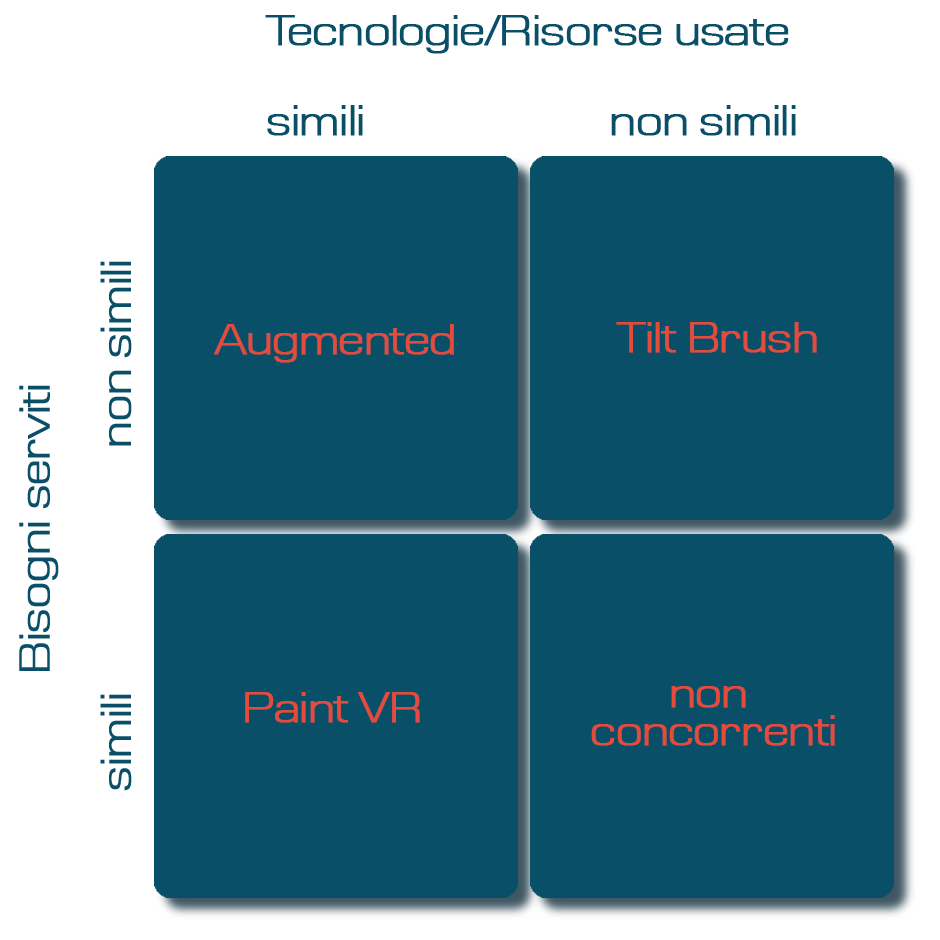
\includegraphics[width=0.60\textwidth]{tabella1.png}
   \caption{Classificazione della concorrenza in base al bisogno servito e le tecnologie usate.}
    \label{fig:awesome_image}
\end{figure}

				
\paragraph{Concorrenti diretti - Paint VR}
Applicazione per Android che, al costo di 4,99 euro , propone all'utente la possibilità di disegnare con un pennello virtuale in uno spazio 3d.\\
Una prima e grossa limitazione di suddetta app, risulta nel supporto agli smartphones: difatti, per poter utilizzare Paint Vr è necessario possedere il visore per la realtà aumentata \textbf{Samsung GearVR} (disponibile in media al prezzo di 100 euro) con cui va accoppiato a uno dei più recenti dispositivi Samsung. Diventa evidente come l'applicazione si stringe in una cerchia di utenti molto stretta (cioè i soli possessori di suddetti dispositivi Samsung).\\
In oltre Paint VR presenta altre importanti limitazioni: 
\begin{itemize}
\item[-] Non offre la possibilità di salvare o esportare i disegni creati, ne tantomeno di condivisione con altri utenti;
\item[-] L'allineamento del controller con il pennello è molto impreciso rendendo l'esperienza utente non solo frustrante, ma anche difficoltosa; 
\item[-] Si presenta con un'interfaccia utente molto minimale, con pennelli basilari e una palette per scegliere il colore. Non è presente lo strumento gomma;
\item[-] Non offre la possibilità di muoversi fisicamente all'interno dei propri disegni, se non mediante il touchpad integrato con il visore;
\end{itemize}
In conclusione, Paint VR risulta essere una buona applicazione per disegnare in realtà virtuale, ma allo stesso tempo uno strumento fine a se stesso e semplicemente ludico.


\paragraph{Concorrenti potenziali - Augment}
E' un'app per smartphones che permette di visualizzare i propri modelli 3D in realtà aumentata, integrati in tempo reale e con le loro reali dimensioni e ambientazione. \\
Tuttavia, funge da solo importatore e visualizzatore di modelli 3d in realtà aumentata.


\paragraph{Concorrenti indiretti- Tilt Brush}
E' un software disponibile a 19,99 euro rilasciato da Google che permette di disegnare in realtà virtuale. \\
Oltre ad offrire un'ampia gamma di pennelli, offre la possibilità di condividere i propri disegni e di salvare delle immagini da diverse angolazioni; \\Di contro, non offre strumenti per la modellazione di oggetti 3d.\\
Per poter usufruire dell'esperienza completa di Tilt Brush serve un visore di realtà virtuale. In una prima fase, il programma era disponibile solo per gli HTC Vive, fattore che poneva già un ostacolo considerando il prezzo di circa 700  euro. Tuttavia adesso è disponibile anche per gli Oculus Rift (disponibili al prezzo di 450 euro). \\
Ovviamente per usare il pennello per disegnare in 3d con TiltBrush, sarà necessario anche possedere dei controllers adeguati per il riconoscimento dei movimenti delle mani.\\
Infine il tutto, ovviamente, deve essere collegato ad un computer e ciò rende non solo Google tiltbrush un'opzione non a portata di tutte le tasche (soprattutto se non si dispone già di un computer sufficientemente potente), ma anche una soluzione estremamente poco portatile.\\

Si può quindi notare come non esistano applicazioni o software in grado di garantire un rapporto bilanciato tra funzionalità, economicità e portatilità del prodotto. Di conseguenza, è possibile ottenere un vantaggio competitivo dalle variabili contingenti che incidono sul consumatore sin dalla percezione del bisogno, quali:
\begin{itemize}
\item[-] Facilità, naturalezza nell'uso degli strumenti da disegno
\item[-] Accesso a strumenti per disegnare a mano libera o per modellare oggetti 3d in un solo posto
\item[-] Economicità del prodotto finale rispetto alle altre proposte sul mercato attuale
\item[-] Portatilità del prodotto finale, niente computer o controller esterni
\item[-] Possibilità di guadagnare visibilità come artista 
\item[-] Possibilità di guadagnare attraverso i propri lavori o acquistarne degli altri
\item[-] Rapporto qualità/prezzo
\end{itemize}

				
%\begin{figure}[h]
%    \centering
%    \includegraphics[width=0.77\textwidth]{ha-gray-conv-crp.jpg}
   % \caption{Picuture of the M83 galaxy, image taken from the WFC3 ERS M83 Data Products, http://archive.stsci.edu/prepds/wfc3ers/m83datalist.html}
   % \label{fig:awesome_image}
%\end{figure}

\section{Posizionamento competitivo}\index{Posizionamento competitivo}
Diversamente dai concorrenti attuali, AirBrush offre una soluzione economica rispetto al prezzo complessivo da dover pagare per un intero set VR, soluzione portatile per lo stesso motivo ed innovativa in quanto alle tecnologie mobili usate; \\
Se gli attuali strumenti di disegno e modellazione in realtà virtuale  non hanno preso troppo piede - o meglio appartengono ad una cerchia ristretta di utenti - è proprio a causa degli elevati costi da affrontare per ottenere il dispositivo finale, composto da svariati elementi, in relazione alla conseguente estrema ingombranza.\\
Infatti, con AirBrush si crede che il mercato mobile sia la chiave dell'adozione di massa del prodotto e la mancanza dell'uso delle mani nelle attuali opzioni VR o AR è l'ingrediente chiave che manca in questo contesto artistico.\\
Inoltre, l'applicazione inizialmente può essere provata in modo totalmente gratuito, seppur con alcune limitazioni , così da costituire una base per l'utente per capire se vuole acquistarla o meno, se non un modo per aumentare la visibilità dell'applicazione.\\
Anche coloro che vogliono semplicemente acquistare i modelli pubblicati da altri utenti nel market di AirBrush  non devono sostenere nessun costo finanziario per farlo, se non quello del modello stesso;\\
Mentre per gli utenti che decideranno di usare AirBrush in modo professionale, dopo la fase di lancio dell'app, dovranno pagare un abbonamento su base annuale (il quale sarà incluso con l'acquisto del visore AR di AirBrush).




%----------------------------------------------------------------------------------------
%	CHAPTER 3
%----------------------------------------------------------------------------------------

\chapterimage{head3.png}
\chapter{Requisiti}

\section{Fattibilità tecnologica}\index{Fattibilità tecnologic}
Per lo sviluppo del prodotto in questione, bisognerà utilizzare linguaggi di programmazione specifici per le app, sia lato iOS che Android;\\ Inoltre bisognerà affidare i dati e la relativa gestione ad un CRM esterno. Questo richiederà innanzitutto che il team di sviluppo sia composto da programmatori qualificati e specializzati nella programmazione di app per entrambi i sistemi operativi;\\
In secondo luogo ci sarà bisogno di far svolgere la parte di CRM a terze parti, almeno nella fase di lancio dell'applicazione, ma anche per guidare il processo di fidelizzazione e l'aumento del Lifetime value (LTV) dei clienti.\\\\
Un altro aspetto riguarda l'utilizzo del visore AR per garantire all'utente un'esperienza immersiva, e del leapmotion per coinvorgerlo interamente nella fase di disegno e per offrire all'artista un'esperienza innovativa, intuitiva e portatile (rendendo in questo modo la società Leap Motion un key partner molto fondamentale).

\begin{figure}[h]
   \centering
    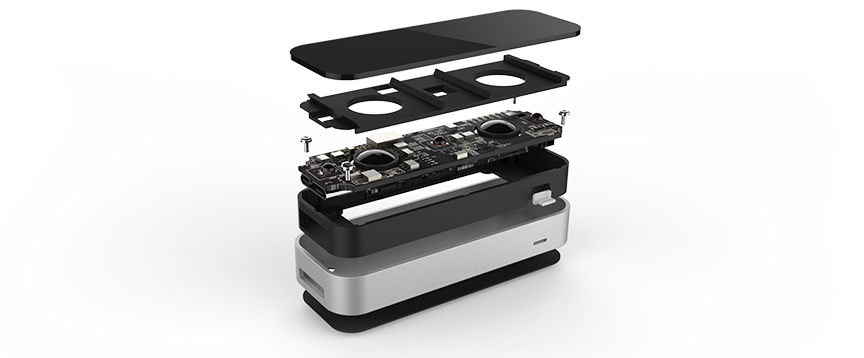
\includegraphics[width=0.60\textwidth]{Leap-Exploded-hero.png}
   \caption{Leap Motion.}
    \label{fig:awesome_image}
\end{figure}

\section{Casi d'uso}
\begin{itemize}
\item\textbf{Viene effettuato l'accesso nell'app ma non si ha connessione internet}
È possibile che un utente acceda all'app senza essere connesso ad alcuna rete dati
o Wi-Fi ed è fondamentale gestire questa situazione in maniera costruttiva affinché
l'utente possa risolvere il problema e proseguire con l'esecuzione dell'applicazione. Al rilevamento di questo evento, l'app notifica l'utente della mancanza ad internet, ma gli permette comunque di creare disegni o moodelli e salvarli in locale. Non gli sarà possibile pubblicarli sul market.

\item\textbf{L'utente scarica l'app dallo store per curiosità}\\
E' possibile che l'utente possa scaricare AirBrush dallo store del suo smartphone per provare il potenziale dell'applicazione, in quanto è un appassionato di disegno e modellazione, o anche per pura e semplice curiosità.\\
In tal caso, come prima schermata gli sarà mostrato un messaggio in cui si raccomanda l'uso di un visore o anche un semplice cardboard associato al telefono e - successivamente - si consiglia l'acquisto del visore per realtà aumentata di AirBrush, per un'esperienza avanzata e fluida dell'applicazione con le proprie mani.
\item\textbf{L'utente decide di abbonarsi}\\
Se l'utente che ha scaricato gratuitamente l'app decide di usarla per scopi professionali in quanto soddisfatto di ciò che offre, sarà ben consapevole che dovrà abbonarsi all'applicazione.\\
Potrà premere il pulsante "Abbonati" presente nella home page, sotto il logo di AirBrush, e sarà rediretto su una schermata in cui potrà decidere quale piano aderisce meglio alle sue esigenze e successivamente, con uno swipe da sinistra verso destra, potrà compilare tutti i dati necessari per l'acquisto dell'abbonamento (come dati personali, carta di credito etc...), mediante l'uso di una tastiera virtuale.\\
Infine, se non lo ha già fatto, gli sarà caldamente consigliato l'acquisto del visore AR di AirBrush, con il quale potrà interagire ad un livello superiore con il proprio spazio di lavoro ed i suoi modelli grazie all'uso del LeapMotion.
\item\textbf{L'utente vuole disegnare qualcosa}\\
L'utente, indossato il visore, si trova nella home page dell'applicazione e da qui preme sul cerchio azzurro con all'interno scritto "Disegna";\\
Se è la prima volta che vi entra, dopo aver scelto con quale mano disegnare (se destra o sinistra) e dopo una breve introduzione alle modalità d'uso dello spazio di disegno ed alle gesture effettuabili con le mani, potrà iniziare a dipingere liberamente nello spazio che lo circonda.\\
L'utente vedrà apparire subito sulla mano degli strumenti le categorie principali dei tools presenti in AirBrush (come disegno a mano libera, modellazione 3d etc..), attraverso le quali potra accedere ai relativi strumenti specifici per quella categoria ed utilizzarli.
\item\textbf{L'utente vuole pubblicare il suo lavoro}\\
L'utente in un qualsiasi momento può salvare il lavoro che sta svolgendo nell'area Disegna, per poterlo riprendere in un secondo momento. Finito il lavoro, l'utente salverà il suo prodotto premendo l'icona "salva" presente nella visuale in alto a destra.\\
Se l'utente è abbonato all'applicazione potrà procedere, altrimenti sarà reindirizzato ad una schermata in cui potrà acquistare un abbonamento per poi poter salvare il lavoro fatto.\\
Successivamente potrà decidere se salvarlo localmente, esportarlo come modello 3d o se pubblicarlo nel Market di AirBrush. Selezionata quest'ultima opzione, l'utente sarà di fronte ad una schermata in cui potrà inserire, attraverso una tastiera virtuale, tutti i dati relativi al progetto come titolo, descrizione e prezzo di acquisto, per poi pubblicarlo sul Market.
\item\textbf{L'utente vuole acquistare un modello dal market}\\
L'utente - che sia abbonato o meno - potrà accedere al market di AirBrush per acquistare i modelli realizzati da altri utenti, premendo sul cerchio rosso con su scritto Market presente nella home page dell'app.\\
Da qui visualizzerà l'intero catalogo dei modelli pubblicati dalla community, visualizzati in ordine di popolarità (visualizzazioni, downloads e punteggi) e suddivisi in categorie (Interior design, abiti, modelli 3d, videogames etc...).\\
Selezionato il modello interessato, l'utente visualizzerà una schermata in cui potrà vedere il modello e camminarci intorno, ruotarlo e spostarlo. A destra sarà presente un pannello con tutti i dati relativi al progetto come autore, titolo, descrizione e prezzo di acquisto.\\
In basso l'utente potrà premere il pulsante Acquista: se l'utente è già abbonato, gli sarà chiesta conferma di acquisto e sarà successivamente scaricato il modello; Altrimenti verrà avvisato del fatto che non potrà utilizzare il modello scaricato in AirBrush, a meno che non acquisti un abbonamento. Se l'utente decide di proseguire senza abbonamento, gli saranno chiesti i dati utili per il pagamento e il modello verrà scaricato.
\end{itemize}




\newpage
%\begin{table}[h]
%  \centering
%  \begin{tabular}{ c c c c c c }
  %  \hline\hline
   % Filter / Config. & Waveband / Central $\lambda$/ Line & Obs. Date & Comment \\
  %  \hline
   % F225W & UV filter / 235.9 nm & 26 Aug 2009 &  UV wide\\
    
  %  F336W & UV filter / 335.5 nm & 26 Aug 2009 & Str$\ddot{o}$mgren $u$\\
    
    %F373N & Narrow-Band Filter / 373.0 nm & 19 Aug 2009 & Includes \textsc{[OII]}\\
    
    %F438W & Wide-Band Filter / 432.5 nm & 26 Aug 2009 & $B$, Johnson-Cousins set\\
    
    %F487N & Narrow-Band Filter / 487.1 nm & 25 Aug 2009 & Includes H$\beta$\\
    
  %  F502N & Narrow-Band Filter / 501.0 nm & 26 Aug 2009 & Includes \textsc{[O III]}\\
    
    %F657N & Narrow-Band Filter / 656.7 nm & 25 Aug 2009 & Includes H$\alpha$+\textsc{[NII]}\\
    
   % F673N & Narrow-Band Filter / 676.6 nm & 20 Aug 2009 & Includes \textsc{[SII]}\\
    
   % F814W & Wide-Band Filter / 802.4 nm & 26 Aug 2009 & $I$, Johnson-Cousins set\\
    %\hline
  %\end{tabular}
  %\caption{Summary of Observations}
 % \label{tab:uno}
%\end{table}

\section{Requisiti per l'esperienza utente}
Di notevole importanza nel prodotto, risulta essere l'esperienza utente. \\L'interfaccia grafica e l'interazione dell'utente con essa avviene interamente all'interno del visore AR e con l'uso delle gesture con le mani come i click per premere pulsanti e gli swipe per andare avanti o indietro.\\
Per quanto riguarda l'area per disegnare, la curva di apprendimento per un utilizzo professionale dell'applicazione sarà molto rapida, proprio grazie alla possibilità di utilizzare le proprie mani per interagire con gli strumenti di lavoro e l'area di disegno. Per ottimizzare il tracking delle mani ed implementare funzionalità più complesse, si è deciso di permettere all'utente di acquistare (con incluso un'abbonamento iniziale) il visore AR AirBrush con integrato il LeapMotion che permetterà un'esperienza utente più fluida ed avanzata.\\

%\begin{remark}
%	Some links to start
%\end{remark}

\section{Conclusione}
In conclusione, AirBrush rappresenta una possibilità innovativa nel campo del Design in qualsivoglia ambito, sia per la sua elevata economicità e portatilità, ma anche in quanto il mercato mobile si presenta ancora privo di prodotti professionali finalizzati alla creazione, condivisione e marketing di modelli e disegni realizzati nel modo più innovativo, intuitivo ed efficiente possibile.
\paragraph{Further work}
Possibili sviluppi del prodotto potranno presentarsi nell'ambito dell'animazione, in cui potranno inserirsi tools per la gestione dei key-frame e tanto altro.

\end{document}
